\documentclass{article}
\usepackage{graphicx} % Required for inserting images
\usepackage[margin=1in]{geometry}
\usepackage{amsmath}
\usepackage{amsthm}
\usepackage{amssymb}
\usepackage{amsfonts}
\usepackage{enumitem}
\usepackage{verbatim}
\usepackage{xcolor}
\usepackage{caption}

\title{Midterm: Report}
\author{Dante Buhl}

\DeclareMathOperator{\cond}{cond}
\DeclareMathOperator{\vecspan}{span}

\begin{document}

\newcommand{\bs}[1]{\boldsymbol{#1}}
\newcommand{\bmp}[1]{\begin{minipage}{#1\textwidth}}
\newcommand{\emp}{\end{minipage}}
\newcommand{\R}{\mathbb{R}}
\newcommand{\C}{\mathbb{C}}
\newcommand{\N}{\mathcal{N}}
\newcommand{\I}{\mathrm{I}}
\newcommand{\K}{\bs{\mathrm{K}}}
\newcommand{\m}{\bs{\mu}_*}
\newcommand{\s}{\bs{\Sigma}_*}
\newcommand{\dt}{\Delta t}
\newcommand{\tr}[1]{\text{Tr}(#1)}
\newcommand{\Tr}[1]{\text{Tr}(#1)}
\newcommand{\hl}[1]{\colorbox{yellow}{#1}}

\maketitle

\section*{Question 1: BVP using Shooting Method and RK4}
\begin{enumerate}[label=\alph*)]

  \item The system can be solved analytically by simply integrating 4 times and
  then solving for the boundary conditions. 
  \begin{align*}
    \int\int\int\int \frac{d^4y}{dx^4} dx^4 &= \int\int\int\int x^2 dx^4\\
    y(x) &= \frac{x^6}{360} + c_1x^3 + c_2x^2 + c_3x + c_4
  \end{align*}
  We can see very clearly from the boundary conditions at $x=0$ that $c_4=c_3=0$.
  We finish solving for $c_1$ and $c_2$.
  \begin{align*}
    0 = \frac{1}{360} + c_1 + c_2, &\quad 0 = \frac{1}{60} + 3c_1 + 2c_2\\
    c_1 = -\frac{1}{90}, &\quad c_2 = \frac{1}{120}
  \end{align*}
  \begin{align*}
    y(x) = \left(\frac{x^6}{360} - \frac{x^3}{90} +
    \frac{x^2}{120}\right)
  \end{align*}

  \item 
  The numerical solution obtained by the shooting method takes the following
  form,
  \begin{align*}
    \frac{dy_1}{dx} &= y_2, \quad y_1(0) = 0\\
    \frac{dy_2}{dx} &= y_3, \quad y_2(0) = 0\\
    \frac{dy_3}{dx} &= y_4, \quad y_3(0) = v_2\\
    \frac{dy_4}{dx} &= x^2, \quad y_4(0) = v_1
  \end{align*}
  Thus we proceed by integrating this ODE with a standard numerical method and
  at each iteration adjust $v_1, v_2$ so that we get closer and closer to the bouncary
  condition at $x=1$. To this end, I will implement something similar to the
  second method. We will update $v_1$ to minimize the error of $y_1$. Then we I
  will update $v_2$ to minimize the error of $y_2$. After iterating several
  times, we obtain accuracy with error at the boundaries less then $10^{-10}$.
  The corresponding initial conditions are $v_1 = -0.066666\ldots$, $v_2 =
  0.016666\ldots$. 

  \item See Fig. 1
    \begin{figure}[ht]
        \centering 
        \begin{minipage}{0.49\textwidth}
            \centering 
            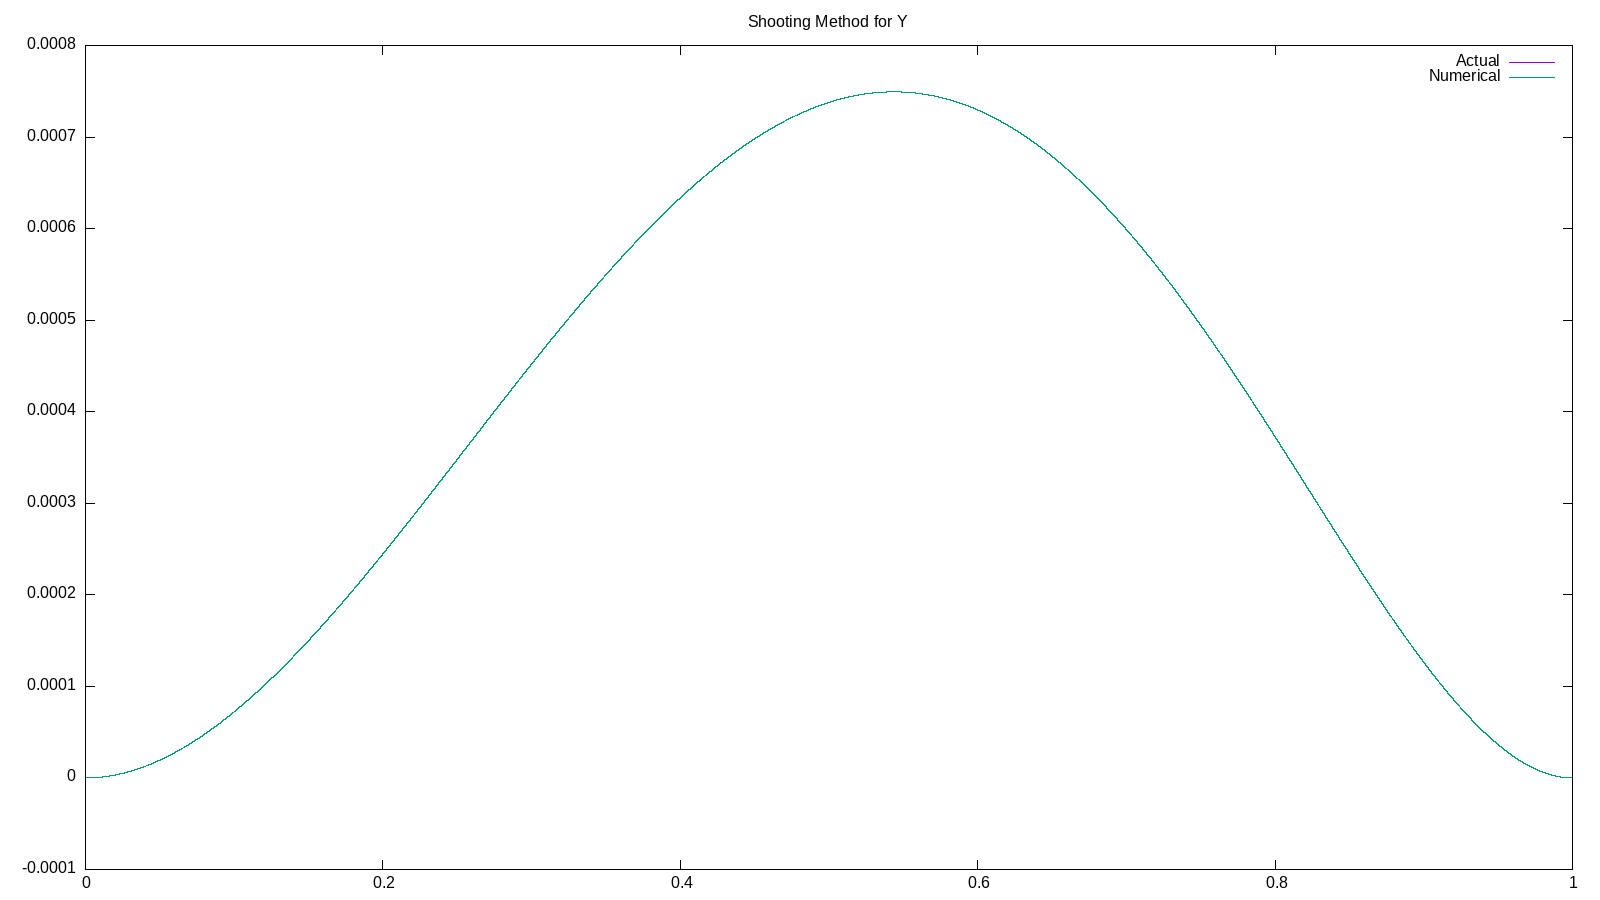
\includegraphics[width=1\textwidth]{rk4_y.png}
            \caption{Numerical Solution for Shooting Method}
        \end{minipage}
        \begin{minipage}{0.49\textwidth}
            \centering 
            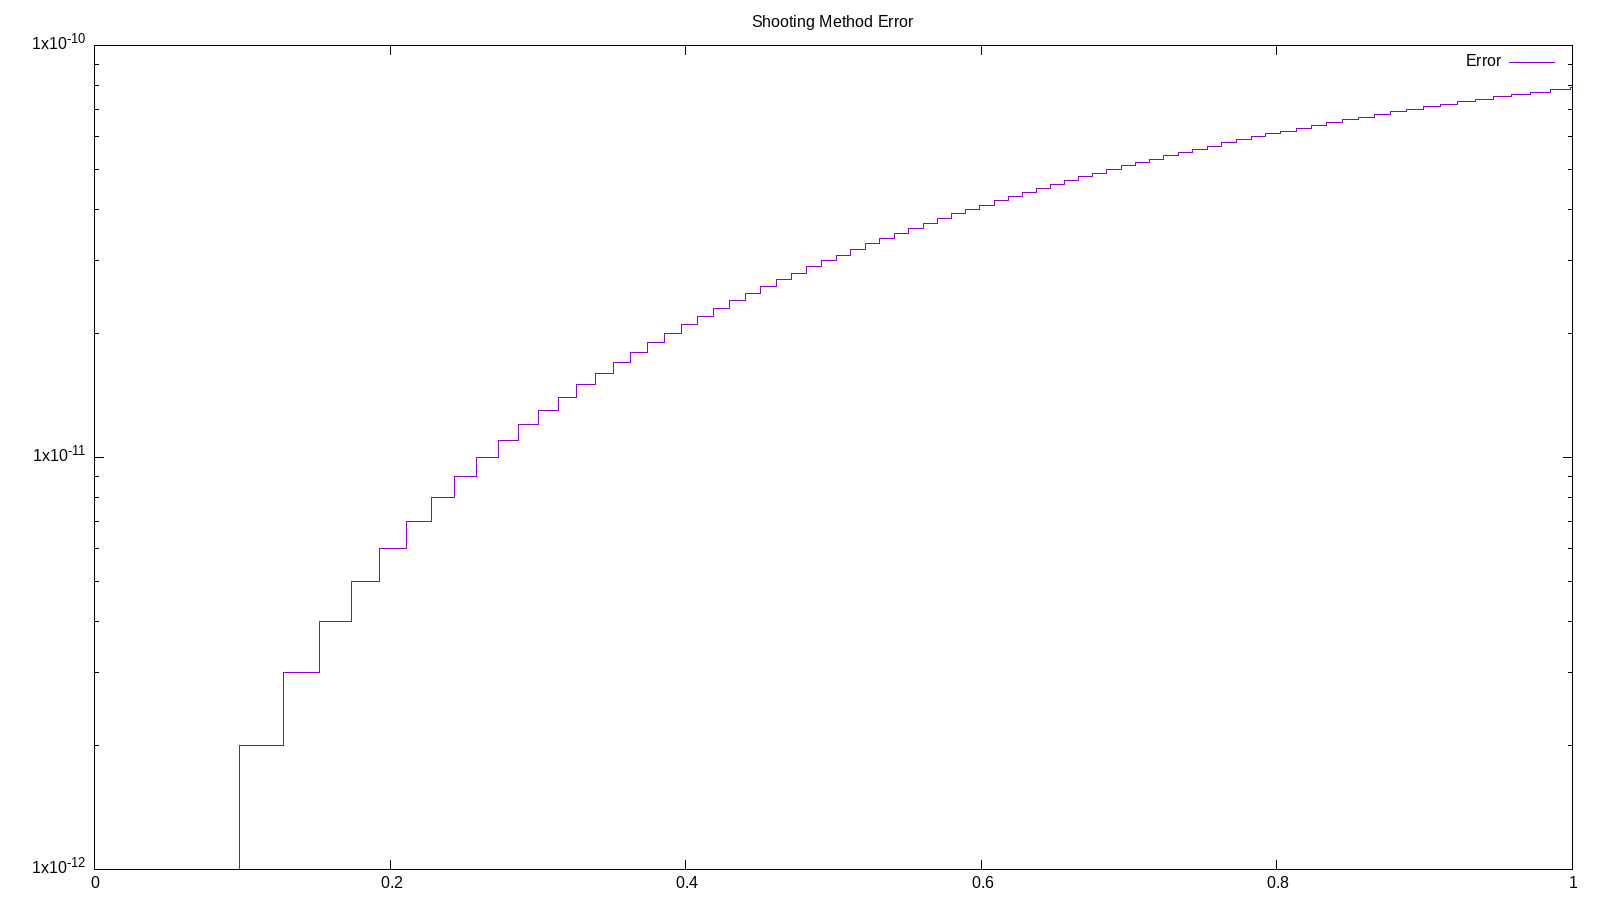
\includegraphics[width=1\textwidth]{rk4_error.png}
            \caption{Numerical Error for Shooting Method}
        \end{minipage}
    \end{figure}

  \item See Fig. 2
        
\end{enumerate}


\section*{Question 2: Convergence and Absolute Stability for an Implicit RK3
Method}

\begin{enumerate}[label=\alph*)]

    \item Prove convergence for Implicit RK3.
    \begin{proof}
        Showing convergence is a matter of showing zero-stability and
        consistency. This is a one-step method, so we have the first
        characteristic polynomial, $\rho(z) = z - 1$. This of course satisfies
        the root condition and therefore is zero-stable. Showing consistency is
        a matter of using a taylor expansion. 
        \begin{align*}
            \bs{y}_{k+1}&=\bs{y}_k + \frac{\dt}{6}\left(\bs{K}_1 + 4\bs{K}_2 +
            \bs{K}_3\right) + \dt\tau_{k+1}\\
            \tau_{k+1}&=\frac{\bs{y}_{k+1}-\bs{y}_k}{\dt} -
            \frac{1}{6}\left(B\bs{y}_k + 4B\left(\bs{y}_k +
            \frac{\dt}{4}\left(\bs{K}_1 + \bs{K}_2\right)\right) 
            +B\left(\bs{y}_k + \dt\bs{K}_2\right)\right)\\
            \tau_{k+1}&=\frac{\bs{y}_{k+1}-\bs{y}_k}{\dt} - \dot{\bs{y}}_k -
            \frac{\dt}{6}B\left(\bs{K}_1 + 2\bs{K}_2\right)
        \end{align*}
        \begin{align*}
            \bs{y}_{k+1} &= \bs{y}_k + \dt\dot{\bs{y}}_k + \dt^2(h.o.t.)\\
            \frac{\bs{y}_{k+1}-\bs{y}_k}{\dt} &=  \dot{\bs{y}}_k + \dt(h.o.t.)\\
            \tau_{k+1}&= -\frac{\dt}{6}B\left(\bs{K}_1 + 2\bs{K}_2\right) +
            \dt(h.o.t.)\\
            |\tau_{k+1}|&= \frac{\dt}{6}\left|B\left(\bs{K}_1 + 2\bs{K}_2\right) +
            \dt(h.o.t.)\right|\\
        \end{align*}
        Thus we have shown consistency with at least order 1, so we must have
        that this Implicit RK3 method is convergent with at least order 1 since
        it is both zero-stable and consistent. 
    \end{proof}

    \item Plot Region of Absolute Statbility (See Fig. 3)
    \begin{figure}[ht]
        \centering 
        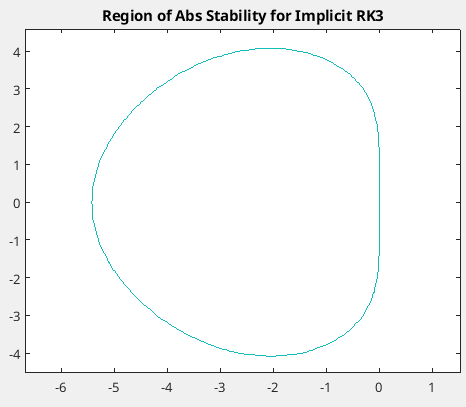
\includegraphics[width=0.5\textwidth]{2.b.AbsStab'.png}
        \caption{Region of Absolute Stability for 2.b.}
    \end{figure}

    \item  
    This problem is solved by plotting the region of absolute stability and
    finding the eignevalues of the matrix B. We notice that since B is an upper
    triangular matrix that its eigenvalues are found on its diagonal. So we have
    that $B$ has all real eigenvalues, $\lambda = \{-1, -2, -4, -16\}$. Next we
    compare to see which eigenvalue is furthest from the region of absolute
    stability. It is evidently the eigenvalue, $\lambda = -16$. So we look at
    the closest point in our region of absolute stability. From the plot we can
    see that the closest point is $\lambda\dt \approx -5.4199 + 0i$. Therefore we
    have that the largest $\dt$ must be, $\dt \approx 0.3387\ldots$. 

    \item As seen in Fig. 4, when $\dt > \dt^*$ we can see that the oscillations
    in the system grow with time while the oscillations for $\dt < \dt^*$ decay
    with time. Ultimately the stability of this method is questionable near
    $\dt^*$, as we can see in the plot of the true solution, however this does
    coincide with the result of absolute stability for this value of $\dt$. To
    remind the reader, the only requirement is for $\bs{u}_k \to 0$ as $k \to
    \infty$
    \begin{figure}[ht]
        \centering 
        \begin{minipage}{0.48\textwidth}
            \centering
            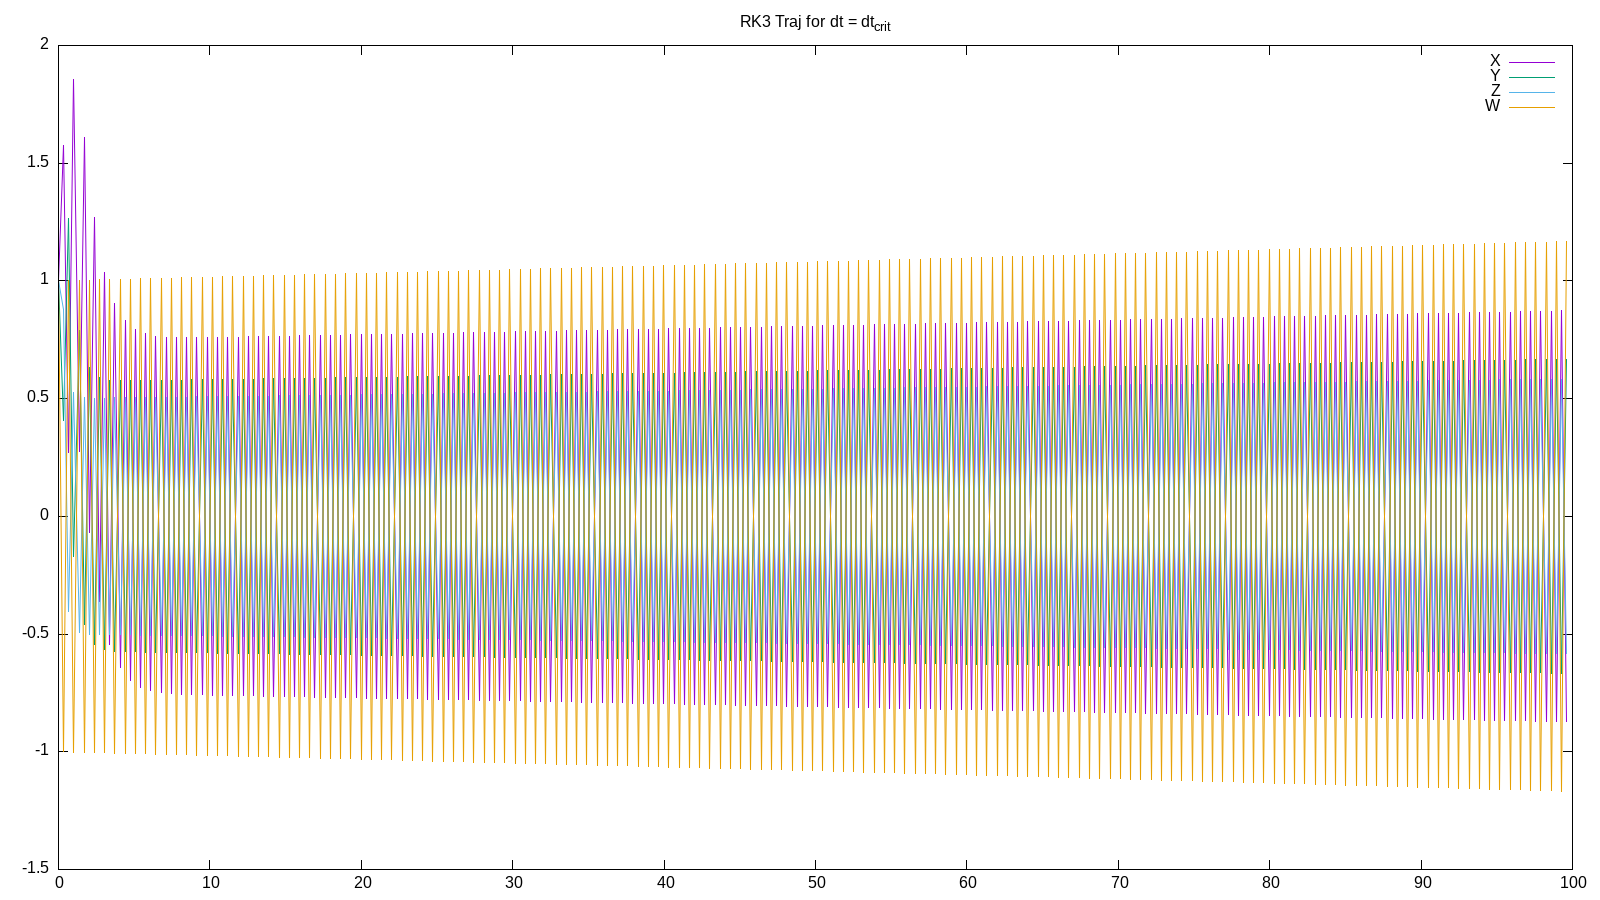
\includegraphics[width=1\textwidth]{rk3_fail.png}
            \caption*{$\dt$ above threshold}
        \end{minipage}
        \begin{minipage}{0.48\textwidth}
            \centering
            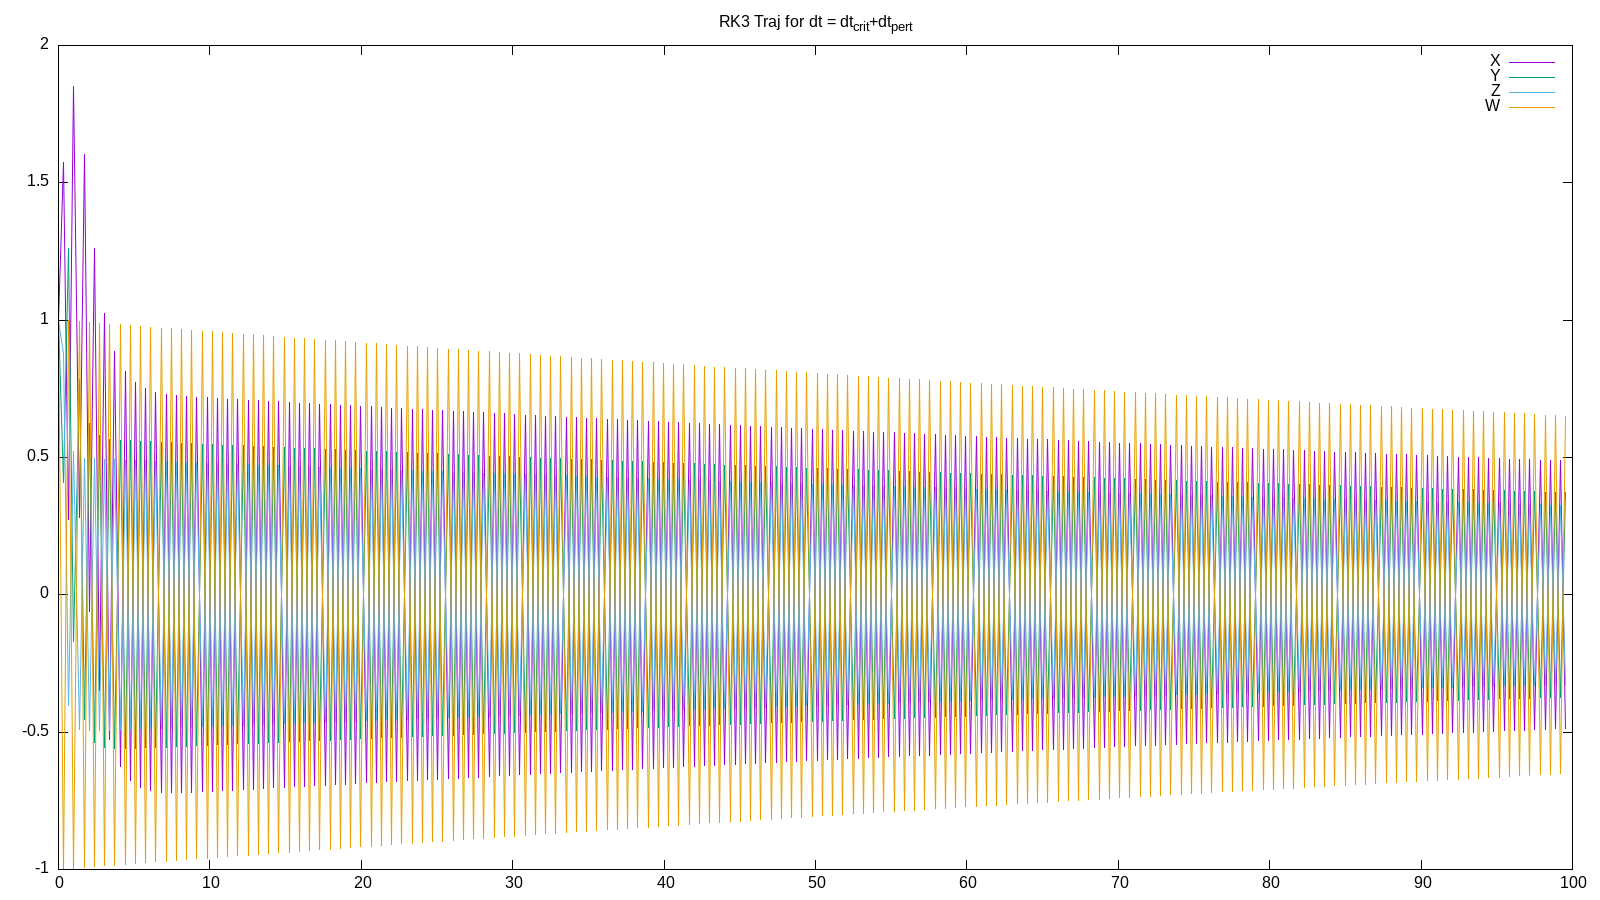
\includegraphics[width=1\textwidth]{rk3_pass.png}
            \caption*{$\dt$ below threshold}
        \end{minipage}
        
        \begin{minipage}{0.6\textwidth}
            \centering
            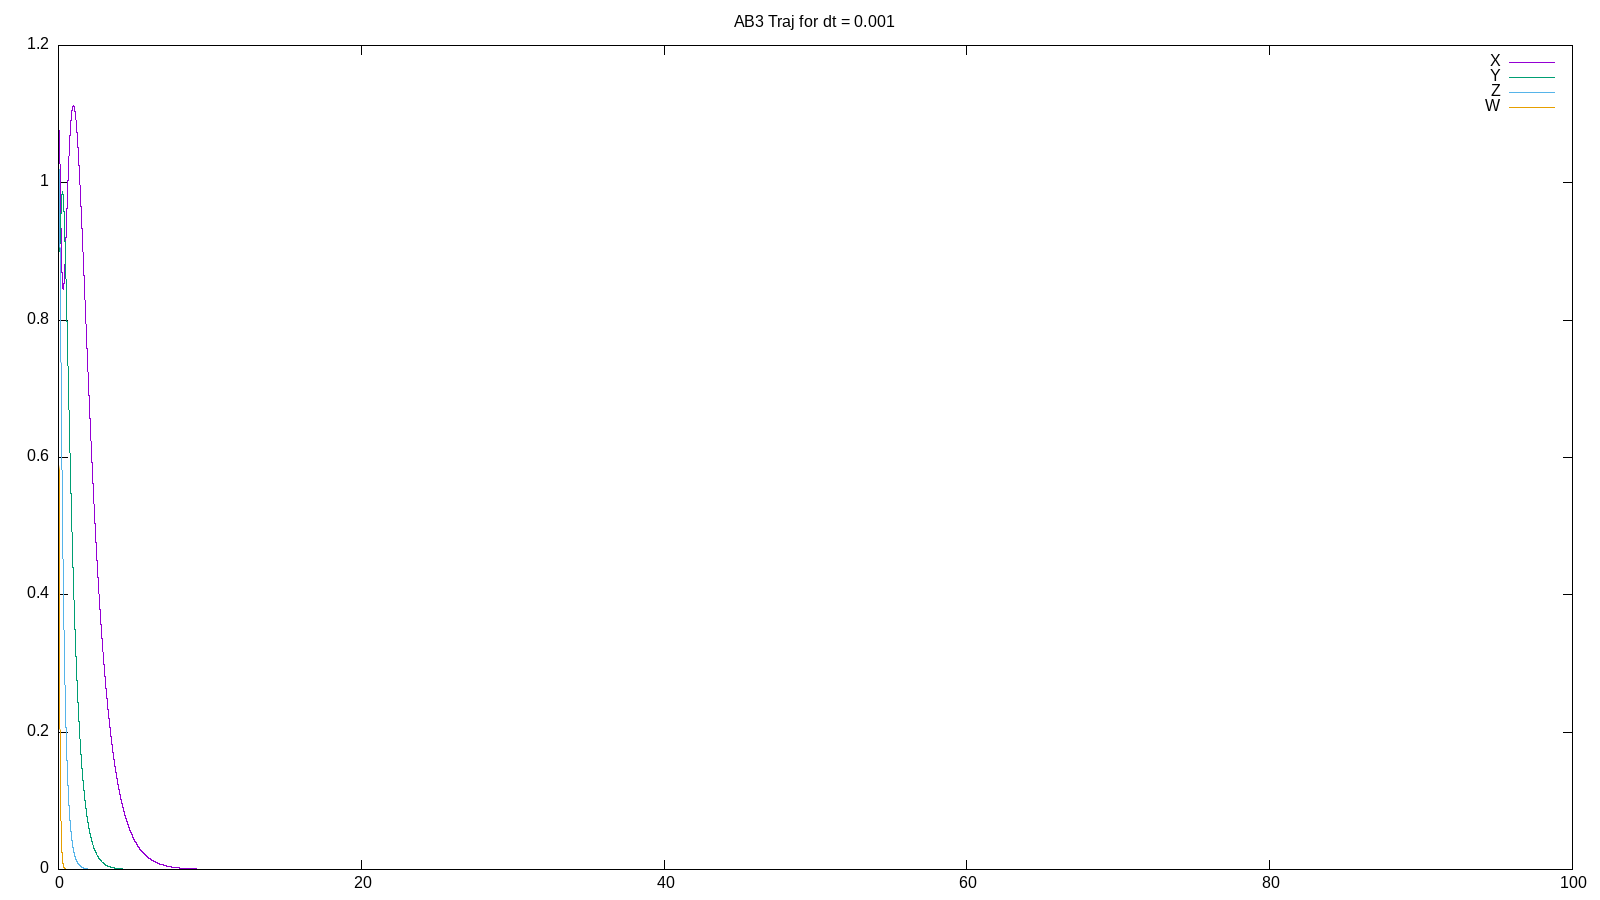
\includegraphics[width=1\textwidth]{rk3_act.png}
            \caption*{True Solution}
        \end{minipage}
        \caption{Evolution of the IC with $\dt$ above and below the calculated
        threshold.}
    \end{figure}

\end{enumerate}

\section*{Question 3: Convergence and Absolute Stability for an LMM}

\begin{align}
    \bs{u}_{k+3} - \frac{1}{3}\left(\bs{u}_{k+2}+\bs{u}_{k+1}+\bs{u}_{k}\right) =
    \frac{\dt}{12}\left[23\bs{f}_{k+2} -2\bs{f}_{k+1} + 3\bs{f}_{k}\right]
\end{align}

\begin{enumerate}[label=\alph*)]

    \item 
    \begin{proof}
        (Zero-Stability)

        We begin this proof first by showing that this LMM is zero-stable. 
        \begin{align*}
            \rho(z) &= z^3 - \frac{1}{3}z^2 - \frac{1}{3}z - \frac{1}{3}\\
            \rho(z) &= (z-1)\left(z^2 + \frac{2}{3}z + \frac{1}{3}\right)\\
            \rho(z) &= (z-1)\left(z - \frac{-\frac{2}{3} \pm \sqrt{\frac{4}{9} -
            \frac{4}{3}}}{2}\right)\\
            \rho(z) &= (z-1)\left(z + \frac{1 \pm i\sqrt{2}}{3}\right)
        \end{align*}
        These are the three complex roots of the characteristic polynomial. We
        now simply must check if all three are within or on the boundary of the
        unit disk. 
        \begin{align*}
            |1| = 1 \le 1, \quad \left|\frac{1 \pm i\sqrt{2}}{3}\right| =
            \frac{1}{9} + \frac{2}{9} = \frac{1}{3} \le 1
        \end{align*}
        As I have just shown, in fact all three roots of the first
        characteristic polynomial fall within the unit disk or on the boundary,
        thus we have that this LMM is zero-stable. 

        (Consistency) 

        We we will look at the consistency of this LMM. We look at the
        definition of truncation error in our system. 
        \begin{align*}
            \bs{y}_{k+3} - \frac{1}{3}(\bs{y}_{k+2} + \bs{y}_{k+1} + \bs{y}_{k}) &=
            \frac{\dt}{12}[\dot{\bs{y}}_{k+2} - 2\dot{\bs{y}}_{k+1} + 3\dot{\bs{y}}_{k}] + \dt
            \tau_{k+3}
        \end{align*}
        In order to simplify this system an demonstrate convergence we will
        convert this problem into terms of $\bs{q}_{k+2}$ using Taylor
        Expansions.
        \begin{align}
            \bs{y}_{k+3} &= \bs{y}_{k+2} + \dt \dot{\bs{y}}_{k+2} +
            \frac{\dt^2}{2}\ddot{\bs{y}}_{k+2} +
            \frac{\dt^3}{6}\dddot{\bs{y}}_{k+2} +
            \frac{\dt^4}{24}\ddddot{\bs{y}}_{k+2} +
            h.o.t.\\
            \bs{y}_{k+1} &= \bs{y}_{k+2} - \dt \dot{\bs{y}}_{k+2} +
            \frac{\dt^2}{2}\ddot{\bs{y}}_{k+2} -
            \frac{\dt^3}{6}\dddot{\bs{y}}_{k+2} +
            \frac{\dt^4}{24}\ddddot{\bs{y}}_{k+2} +
            h.o.t.\\
            \bs{y}_{k+1} &= \bs{y}_{k+2} - 2\dt \dot{\bs{y}}_{k+2} +
            \frac{4\dt^2}{2}\ddot{\bs{y}}_{k+2} -
            \frac{8\dt^3}{6}\dddot{\bs{y}}_{k+2} +
            \frac{16\dt^4}{24}\ddddot{\bs{y}}_{k+2} +
            h.o.t.\\
            \dot{\bs{y}}_{k+1} &= \dot{\bs{y}}_{k+2} - \dt \ddot{\bs{y}}_{k+2} + 
            \frac{\dt^2}{2}\dddot{\bs{y}}_{k+2} -
            \frac{\dt^3}{6}\ddddot{\bs{y}}_{k+2} + h.o.t\\
            \dot{\bs{y}}_{k} &= \dot{\bs{y}}_{k+2} - 2\dt \ddot{\bs{y}}_{k+2} + 
            \frac{4\dt^2}{2}\dddot{\bs{y}}_{k+2} -
            \frac{8\dt^3}{6}\ddddot{\bs{y}}_{k+2} + h.o.t
        \end{align}
        Using this we can build a linear system to satisfy order 1 consistency,
        then we can check to see if any of the other orders happen to be
        satisfied by the solution. If the following system has a solution then we
        have, 
        \begin{align*}
            \left[\begin{array}{c c c}1 & -1/3 & -1/3 \\ 1 & 1/3 & 2/3 \\ 1/2 &-1/6 &
            -2/3\end{array}\right]
            \left[\begin{array}{c}A\\B\\C \end{array}\right]
            =
            \left[\begin{array}{c}1/3\\2\\-1/3 \end{array}\right]
            \implies \tau_{k+3} = C\dt^2
        \end{align*}
        Furthermore, if we can show that these coefficients satisfy higher order
        equations then we can demonstrate higher order convergence. As it
        happens, the solution to this system is, $A = B = C = 1$. Thus we have
        that this system is at least consistent with order 2, and thus at least
        convergent with order 2 since zero-stability was already implied. So we look at
        the higher orders of convergence/consistency. 
        \begin{align*}
            \left[\begin{array}{c c c}1/6 & 1/18 & 8/18 \\ 1/24 & -1/72 & -16/72 \end{array}\right]
            \left[\begin{array}{c}A\\B\\C \end{array}\right]
            i&\stackrel{?}{=}
            \left[\begin{array}{c}5/12\\-2/9 \end{array}\right]\\
            \left[\begin{array}{c c c}1/6 & 1/18 & 8/18 \\ 1/24 & -1/72 & -16/72 \end{array}\right]
            \left[\begin{array}{c}A\\B\\C \end{array}\right]
            - 
            \left[\begin{array}{c}5/12\\-2/9 \end{array}\right] &= 
            \left[\begin{array}{c}0.2499\ldots\\-5.40277\ldots \end{array}\right]
        \end{align*}
        Thus no higher order of convergence is obtained. Therefore this system
        is convergence with order 2. 
    \end{proof}

    \item Absolute Stability and A-Stability

    We can plot the region of absolute stability for this LMM. We have the first
    and second characterstic polynomials are the following. 
    \begin{align*}
        \rho(z) = z^3 - \frac{1}{3}\left(z^2 + z + 1\right), &\quad \sigma(z) =
        \frac{1}{12}\left(23z^2 - 2z + 3\right)\\
        \frac{\rho(z)}{\sigma(z)} = \lambda \dt 
    \end{align*}
    We can then plot this by evaluating $\frac{\rho(z)}{\sigma(z)}$ with
    $z=e^{i\theta}$ and plotting in the complex plane. 
    \begin{figure}[h]
        \centering 
        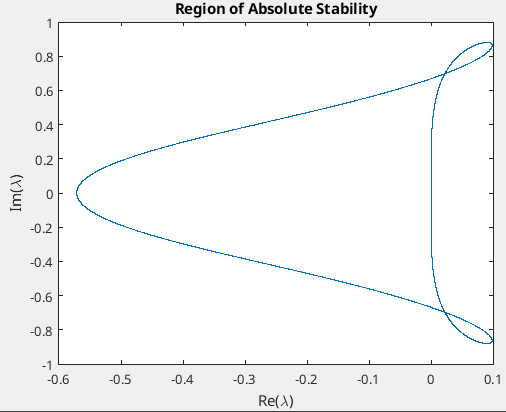
\includegraphics[width=0.5\textwidth]{3.b.AbsStab.png}
        \caption{Region of Absolute Stability for 3.b}
    \end{figure}
    We can see from this plot that this LMM is certainly not A-Stable. The
    reason being that the region of absolute stability is only conditionally
    absolutely stable. This is seen in the plot which clearly illurstrates the
    region of absolute stability including only a small subset of $\C^-$. 
    

\end{enumerate}

\end{document}
